\documentclass[12pt]{article}
\usepackage{graphicx,verbatim}
\setlength{\topmargin}{-.8 in}
\setlength{\textheight}{9.4  in}
\setlength{\oddsidemargin}{-.1in}
\setlength{\evensidemargin}{-.1in}
\setlength{\textwidth}{6.35in}
 \usepackage{graphicx}
 \usepackage{algpseudocode}
 \usepackage{algorithm}
 \usepackage{amsmath}

\include{macros}
\begin{document}

\begin{center}
\large{CS591 P3}
\end {center}

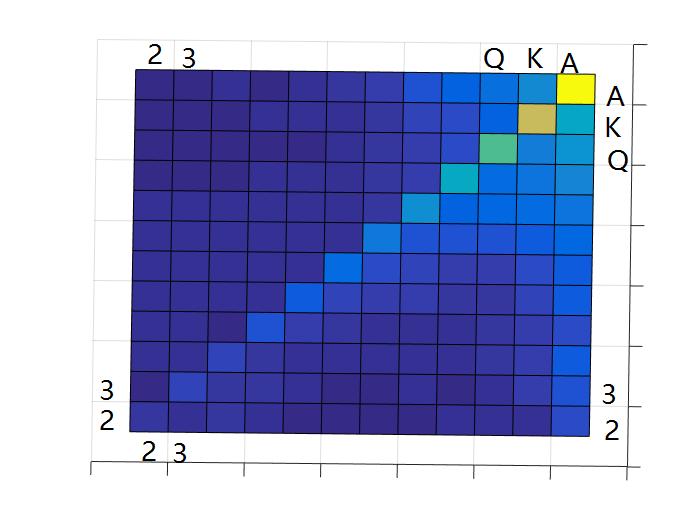
\includegraphics[scale=.5]{score}
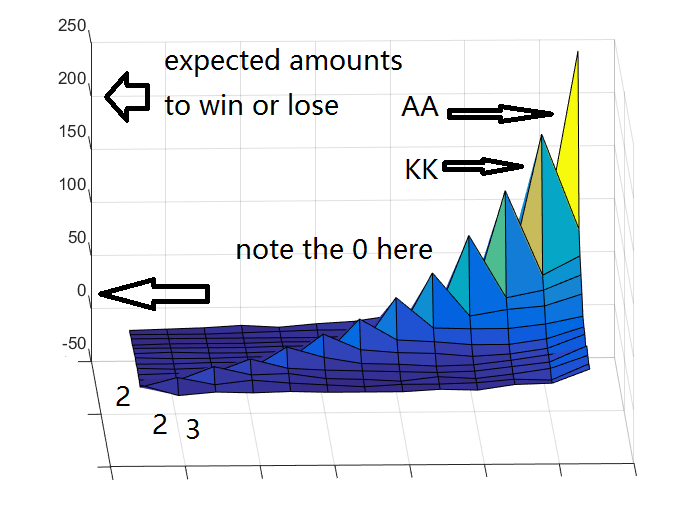
\includegraphics[scale=.5]{score1}

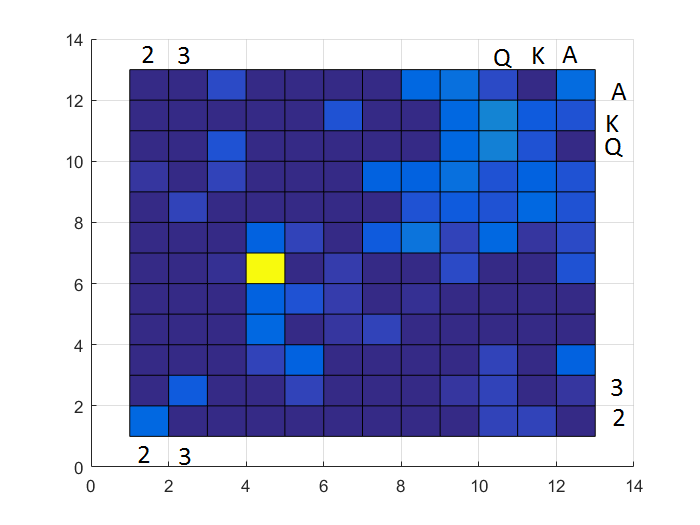
\includegraphics[scale=.5]{A0mR}
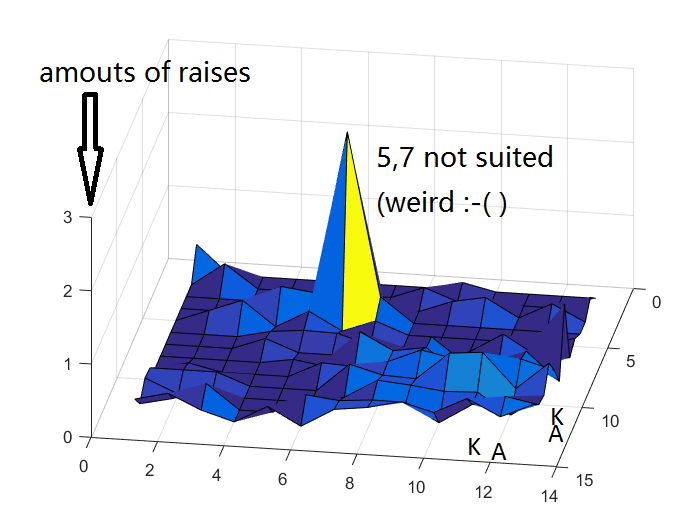
\includegraphics[scale=.5]{A0mR1}

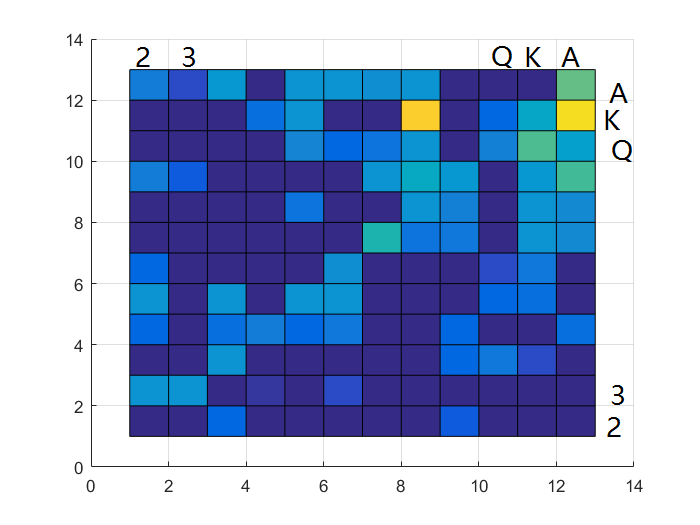
\includegraphics[scale=.5]{B0mR}
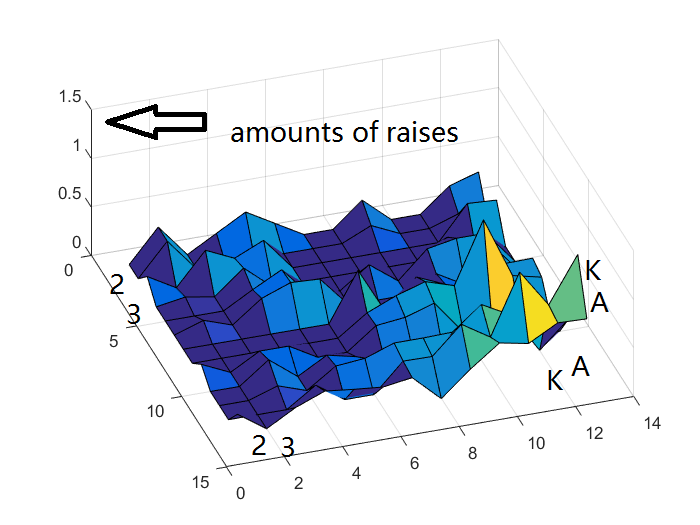
\includegraphics[scale=.5]{B0mR1}

The above four figures are about the same player whose hands are randomly partitioned into two sets. The Hausdorff distance between the two shapes is 2.5583.

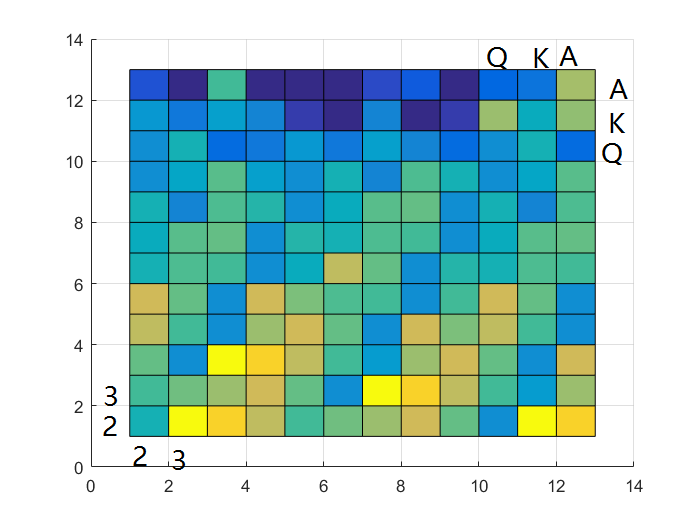
\includegraphics[scale=.5]{AEL5}
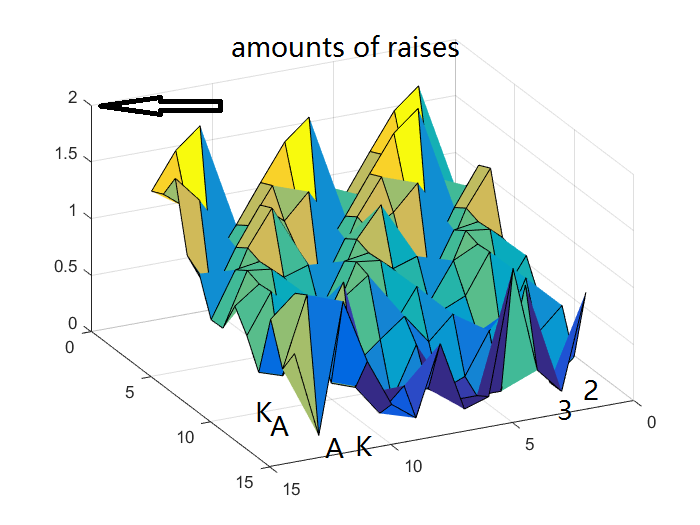
\includegraphics[scale=.5]{AEL51}

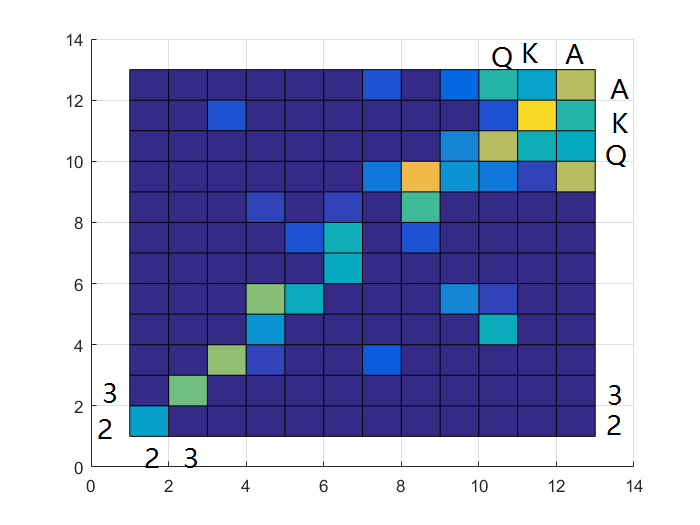
\includegraphics[scale=.5]{BEL5}
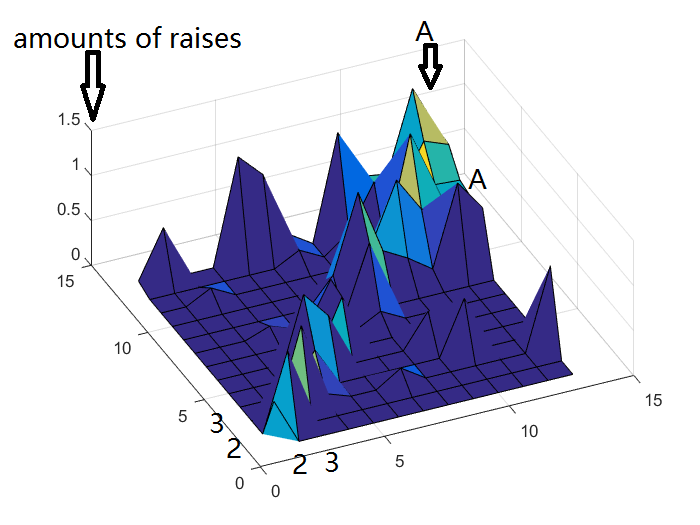
\includegraphics[scale=.5]{BEL51}

The above four figures are about the same player whose hands are randomly partitioned into two sets. The Hausdorff distance between the two shapes is 1.1667.


CHALLENGES 

Opposed to what we expected before, we don't actually have enough data of some players. This might explain in part why there are quite a few players don't have a consistent play pattern. If we don't have a stabilized data set in a meaningful way, we can't simply apply the Hausdorff distance to summarize the pattern of a player, as we assume that the Hausdorff distance has to be smaller within a player than across players, is the distance is a good metric for their summaries.

In order to simplify the patterns,
our tentative analysis excluded human interaction mostly which, in fact, plays a major role in gaming. However, to include human interaction would make the patterns less stable and tangible. Given that the data size is not even good enough for a compromised analysis, we don't really know if it'd be too much to ask for deeper analysis on human interaction.




 
        
  
 

\end{document}